\PassOptionsToPackage{sols}{handout}
\documentclass[main]{subfiles}
\setcounterrefbeforedot{chapter}{m-ws1-3}
\setcounterrefafterdot{section}{m-ws1-3}
\addtocounter{section}{-1}
\usepackage{solutions}

\begin{document}

\section{More Related Rates Problems} \label{ws1-3}

% \begin{objectives}

% Learning Objectives:

% \begin{itemize}[topsep=0pt,partopsep=0pt,parsep=8pt,itemsep=0pt]

% \item You should be able to solve problems relating rates of change.

% \item You should be able to interpret your solutions and check that they
%   make sense in the context of a related rates problem. 

% \item You should appreciate how related rates problems are applications of
%   the Chain Rule and implicit differentiation. 

% \end{itemize}
% \end{objectives}

\begin{enumerate}
\item  %({{{Problem Set 4}, {{{{\#6}}(b)}}}})
 % based on Gottlieb 17.4.14

  Thabo is working on the following problem:
  \begin{quote}
    It is evening and a 5-foot-tall woman is standing by a 15-foot-high
    street lamp on a cobbled road, waiting for a friend to pick her up.
    When she sees her friend pull her car up to the curb she begins to
    walk away from the light at a rate of 4 feet per second.  How fast
    is the length of her shadow changing?
  \end{quote}
  Thabo has drawn the following picture and labeled some variables but is
  unsure what to do next.

  \begin{center}
    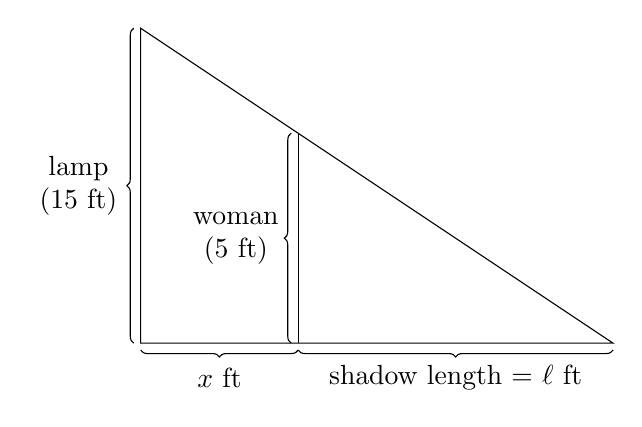
\begin{tikzpicture}[x=1cm, y=1cm]
      \draw (0, 0) -- (-6, 0) -- (-6, 4) -- cycle;
      \draw (-4, 0) -- (-4, 8/3);
      \draw[decorate, decoration={brace, mirror}, yshift=-.25em] (-6,
      0) -- node[midway, yshift=-1em]{$x$ ft} (-4,0);
      \draw[decorate, decoration={brace, mirror}, yshift=-.25em] (-4,0) --
      node[midway, yshift=-1em]{shadow length = $\ell$ ft} (0,0); 
      \draw[decorate, decoration={brace}, xshift=-.25em] (-6,0) --
      node[midway, xshift=-2em, text width=3em, text centered]{lamp (15
        ft)} (-6,4);  
      \draw[decorate, decoration={brace}, xshift=-.25em] (-4,0) --
      node[midway, xshift=-2em, text width=4em, text centered]{woman (5 ft)} (-4,8/3); 
    \end{tikzpicture}
  \end{center}



  \begin{enumerate}
  \item
    Thabo knows it's always a good idea to start by figuring out your
    goal and what you know, so he's trying to do that.  Which of the
    following best describes the problem Thabo is trying to solve in
    terms of time $t$ and the variables $x, \ell$ in the picture?
    
      \begin{multicols}{2}
      \begin{enumerate}[label=\protect\maybecircle{\Alph*.}]
      \plainitem Goal: Find $\dfrac{d\ell}{dx}$ when $x = 4$.
      \plainitem Goal: Find $\dfrac{d\ell}{dt}$ when $x = 4$.
      \plainitem Goal: Find $\dfrac{dx}{dt}$ when
        $\dfrac{d\ell}{dt} = 4$.
      \circleitem Goal: Find $\dfrac{d\ell}{dt}$ when
        $\dfrac{dx}{dt} = 4$. 
      \end{enumerate}
      \end{multicols}
    
  \item
    \begin{problem}[\vfill]
      Write down an equation relating $x$ and $\ell$.  (\emph{Hint:} Use
      similar triangles!)
    \end{problem}

    \begin{solution}
      The red and green triangles below are similar; this is the case
      because they share an angle (the lower right angle) and the red and
      green sides opposite this angle are parallel (both vertical): 
      \begin{center}
        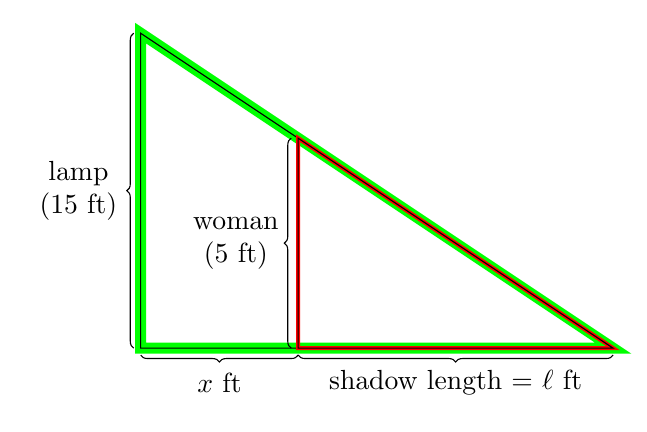
\begin{tikzpicture}[x=1cm, y=1cm]
          \draw[line width=4pt, green] (0, 0) -- (-6, 0) -- (-6, 4) -- cycle;
          \draw (0, 0) -- (-6, 0) -- (-6, 4) -- cycle;
          \draw[line width=1.5pt, red] (0, 0) -- (-4, 0) -- (-4, 8/3) -- cycle;
          \draw (-4, 0) -- (-4, 8/3) -- (0, 0) -- cycle;
          \draw[decorate, decoration={brace, mirror}, yshift=-.25em] (-6,
          0) -- node[midway, yshift=-1em]{$x$ ft} (-4,0);
          \draw[decorate, decoration={brace, mirror}, yshift=-.25em] (-4,0) --
          node[midway, yshift=-1em]{shadow length = $\ell$ ft} (0,0); 
          \draw[decorate, decoration={brace}, xshift=-.25em] (-6,0) --
          node[midway, xshift=-2em, text width=3em, text centered]{lamp (15
            ft)} (-6,4);  
          \draw[decorate, decoration={brace}, xshift=-.25em] (-4,0) --
          node[midway, xshift=-2em, text width=4em, text centered]{woman (5 ft)} (-4,8/3); 
        \end{tikzpicture}
      \end{center}
      Therefore, the two triangles have the same ratio of height to width;
      that is, $\frac{5}{\ell} = \frac{15}{x + \ell}$.  If you like, you
      could rewrite this equation without fractions by cross-multiplying:
      $5 (x + \ell) = 15 \ell$.
    \end{solution}

  \item
    \begin{problem}[\nstretch{2}]
      Solve this problem.
    \end{problem}

    \begin{solution}
      In {{{{\#1}}(b)}}, we found the equation $5(x +
      \ell) = 15 \ell$.  Taking the derivative of both sides with respect
      to $t$,
      \begin{align*}
        \frac{d}{dt} \Big[ 5 (x + \ell) \Big] &= \frac{d}{dt} (15 \ell) \\
        5 \left( \frac{dx}{dt} + \frac{d\ell}{dt} \right) &= 15
        \frac{d\ell}{dt} \\
        \intertext{We know that $\frac{dx}{dt} = 4$:}
        5 \left( 4 + \frac{d\ell}{dt} \right) &= 15 \frac{d\ell}{dt} \\
        20 &= 10 \frac{d\ell}{dt} 
      \end{align*}
      So, $\frac{d\ell}{dt} = \boxed{2 \text{ feet per second}}$.

      \checkmark{} It makes sense that $\frac{d\ell}{dt}$ is positive since
      $\ell$ is increasing. 
    \end{solution}

  \end{enumerate}

\item 
  % Adapted from Juliana' worksheet, which was adapted from stewart and
  % Gottlieb, 17.4, 17.10

      Your calculus book is sitting on your desk, leaning against the wall
      as shown.  The book is slowly sliding down the wall. At the moment
      shown in the snapshot on the left, the top of the book is sliding down 
      at a rate of 1 inch per second.  Find the (instantaneous) rate at 
      which the bottom of the book is sliding along the desk at that moment.

      \begin{figure}[H]\centering
      \begin{tabular}{cc}
      \begin{tikzpicture}[x=0.3cm, y=0.3cm]
          \coordinate (top) at (0, 10);
          \coordinate (bottom) at (2, 0);
          \draw (0, 0) -- (0,12);
          \draw (0, 0) -- (5,0);        
          \draw[fill=lightgray] let \p1 = ($(top)+(bottom)$),
          \n2={4pt/veclen(\x1, \y1)} in (top) -- (bottom) -- ($(bottom) +
          (\n2*\y1, \n2*\x1)$) -- ($(top)+ (\n2*\y1, \n2*\x1)$) -- cycle;
          \draw[|-|] (0, -6pt) -- node[below]{$2$} ($(bottom)-(0, 6pt)$);
          \draw[|-|] (-6pt, 0) -- node[left]{$10$} ($(top)-(6pt, 0)$);        
      \end{tikzpicture} \hspace{120pt} &
      \solonly{\begin{tikzpicture}[x=0.3cm, y=0.3cm]
          \coordinate (top) at (0, 7.4);
          \coordinate (bottom) at (7, 0);
          \draw (0, 0) -- (0,12);
          \draw (0, 0) -- (9,0);        
          \draw[fill=lightgray] let \p1 = ($(top)+(bottom)$),
          \n2={4pt/veclen(\x1, \y1)} in (top) -- (bottom) -- ($(bottom) +
          (\n2*\y1, \n2*\x1)$) -- ($(top)+ (\n2*\y1, \n2*\x1)$) -- cycle;
          \draw[|-|] (0, -6pt) -- node[below]{$x$} ($(bottom)-(0, 6pt)$);
          \draw[|-|] (-6pt, 0) -- node[left]{$y$} ($(top)-(6pt, 0)$);
          \draw ($0.5*(top)+0.5*(bottom)$) node[anchor=south west]
          {$\sqrt{104}$}; 
        \end{tikzpicture}}
      \probonly{\begin{tikzpicture}[x=0.3cm, y=0.3cm]
          \coordinate (top) at (0, 7.4);
          \coordinate (bottom) at (7, 0);
          \draw (0, 0) -- (0,12);
          \draw (0, 0) -- (9,0);        
          \phantom{\draw[|-|] (0, -6pt) -- node[below]{$x$} ($(bottom)-(0, 6pt)$);}
          \phantom{\draw[|-|] (-6pt, 0) -- node[left]{$y$} ($(top)-(6pt, 0)$);}
        \end{tikzpicture}}
      \end{tabular}
      \end{figure}
      
      \begin{enumerate}
      \item
        \begin{problem}
        The diagram drawn on the left is a ``snapshot'' showing the book at a particular moment in time.  Draw a ``general'' diagram on the right which could apply at any time. (Use variables for quantities that are changing over time, and only use concrete values for quantities that are constant.)
        \end{problem}

    \begin{solution}
        The top of the book is sliding down, and the bottom of the book is
        sliding to the right.  Therefore, the two distances shown in the
        picture are changing.  On the other hand, the actual size of the
        book is constant: by the Pythagorean Theorem, the height of the
        book itself is $\sqrt{104}$ inches. 
      \end{solution}

    \item
      \begin{problem}[\stretch{0.5}]
        What's the goal in this problem?  (What rate are you looking for?)
      \end{problem}

      \begin{solution}
        We are looking for the instantaneous rate at which the bottom of
        the book is sliding, or $\frac{dx}{dt}$. 
      \end{solution}

    \item
      \begin{problem}[\stretch{0.5}]
        What information do you know because it's given in the problem?
      \end{problem}

      \begin{solution}
        We are told that the top of the book is sliding down at a rate of
        1 inch per second, so $\frac{dy}{dt} = -1$ (this rate is negative
        because $y$ is decreasing). 
      \end{solution}

    \item
      \begin{problem}[\stretch{0.5}]
        What relationships can you come up with among your variables?
        Write an equation that relates your variables.
      \end{problem}

      \begin{solution}
        By the Pythagorean Theorem, $x^2 + y^2 = 104$. 
      \end{solution}

    \item
      \begin{problem}[\stretch{2}]
        Differentiate both sides of your equation and solve for the rate you're looking for.
      \end{problem}

      \begin{solution}
        We figured out in {{{{\#2}}(d)}} that
        \begin{align}
          x^2 + y^2 &= 104 \nonumber \\
          \intertext{Let's differentiate this equation with respect to $t$
            (since we're looking for $\frac{dx}{d\ideas{\bm{t}}}$):} %
          2x \frac{dx}{dt} + 2y \frac{dy}{dt} &=
          0
 \\
          \intertext{At the moment we are interested in, $x = 2$, $y =
            10$, and $\frac{dy}{dt} = -1$:}
          2 (2) \frac{dx}{dt} + 2 (10)(-1) &= 0 \nonumber 
        \end{align}
        Solving, $\frac{dx}{dt} = 5$ inches per second.
      \end{solution}

    \note{Matt note - encourage them to unpack "constant rate." Students will often read this and skip past the fact this tells the derivative is 0.}

    \item
      \begin{problem}[\vfill\newpage]
        If the top of the book continues to slide down the wall at a constant rate of 1 inch per second, does the bottom of the book slide to the right at a constant rate?  If not, how does this rate change?  Explain by finding a formula for the rate at which the bottom of the book slides to the right. 
      \end{problem}

      \begin{solution}
        Equation (1) is always true (we didn't
        plug in any of the snapshot information until after we got this
        equation).  That is, it's always true that $2x \frac{dx}{dt} + 2y
        \frac{dy}{dt} = 0$.  If, in addition, $\frac{dy}{dt}$ is always
        equal to $-1$, then $2x \frac{dx}{dt} - 2y = 0$, so $\frac{dy}{dt}
        = \frac{y}{x}$.  As the book slides, $y$ decreases and $x$
        increases, so $\frac{dx}{dt} = \frac{y}{x}$ decreases (gets closer
        to 0) as time goes on.  That is, \fbox{the bottom of the book
          slides more slowly as time goes on}.
      \end{solution}

    \end{enumerate}

\end{enumerate}

\begin{framed}
    \textbf{General Strategy for Related Rates Problems}
    \begin{enumerate}
        \item \textbf{Understand the problem} by drawing diagrams and identifying variables, momentary values of those variables, and constants. You may want to draw a snapshot diagram and a general diagram. Write down the rate(s) given to you and determine which rate you need to find.
        \item \textbf{Relate the variables} whose rates are given with the variable whose rate you need to find. This may involve using geometric formulas, the Pythagorean theorem, similarity, etc.
        \item \textbf{Differentiate both sides} with respect to time to get a relationship between the rates.
        \item \textbf{Plug in values} for all variables and rates other than the rate you need to find. Make sure to use values from the correct moment in time. If you are missing values, solve for them using the original relationship between the variables or by coming up with another relationship.
        \item \textbf{Solve for the rate} you need to find. Check if the value seems reasonable, especially the sign.
    \end{enumerate}
\end{framed}

\begin{enumerate}[resume]

\item 
    % stolen from Peter Garfield

    \note{Students will need to be careful here about the signs of the
      given rates.  It's common for students to think that things
      traveling north and east automatically have positive rates; help
      them realize that, since their variables probably represent
      distances, they should be thinking about whether those distances are
      increasing or decreasing.}

    \begin{problem}[\nstretch{3}]
      Two cars are approaching an intersection. A red car, approaching
      from the north, is traveling 20 feet per second and is currently 60
      feet from the intersection. A blue car, approaching from the west,
      is traveling 30 feet per second and is currently 80 feet from the
      intersection.  At this moment, is the distance between the two cars
      increasing or decreasing?  How quickly?
    \end{problem}

    \begin{solution}
      Intuitively, since both cars are heading toward the intersection,
      they are getting closer to each other, so the distance between the
      two cars should be decreasing.

      At the moment described in the problem, the situation looks like
      this (the red and blue car are represented by dots; the intersection
      is the $+$):
      \begin{center}
        \begin{tikzpicture}[x=0.05cm, y=0.05cm]
          \draw (0, 60) -- node[right] {60} (0, 0) -- node[below] {80} (-80,
          0);
          \draw[very thick] (2, 0) -- (-2, 0);
          \draw[very thick] (0, 2) -- (0, -2);
          \draw[red, fill=red] (0, 60) circle(2pt);
          \draw[blue, fill=blue] (-80, 0) circle(2pt);
          \draw[red, ->, xshift=-4pt] (0, 60) -- node[left]{20 ft/s} (0,
          50);
          \draw[blue, ->, yshift=4pt] (-80, 0) -- node[above]{30 ft/s}
          (-70, 0); 
        \end{tikzpicture}

        \emph{Snapshot}
      \end{center}
      However, the most important picture to draw is the ``generic'' one
      that shows how the situation could look at an arbitrary time.
      Here's a generic picture for this situation.  We've labeled some
      variables in it: $x$ for the blue car's distance from the
      intersection and $y$ for the red car's distance from the
      intersection.
      \begin{center}
        \begin{tikzpicture}[x=0.05cm, y=0.05cm]
          \draw (0, 60) -- (0, 0) -- (-80, 0);
          \draw[very thick] (2, 0) -- (-2, 0);
          \draw[very thick] (0, 2) -- (0, -2);
          \draw[red, fill=red] (0, 30) circle(2pt);
          \draw[blue, fill=blue] (-60, 0) circle(2pt);
          \draw[red, thick] (0, 0) -- (0, 30);
          \draw[blue, thick] (0, 0) -- (-60, 0);
          \draw[red, decorate, decoration={brace, mirror}, xshift=4pt] (0,
          0) -- node[midway, xshift=1em]{$y$} (0, 30);  
          \draw[blue, decorate, decoration={brace}, yshift=-4pt] (0,
          0) -- node[midway, yshift=-1em]{$x$} (-60, 0);  
        \end{tikzpicture}

        \emph{Generic}
      \end{center}

      \ideas{Next, we figure out what we know and what we want to know.}

      \highlight{ \textbf{What we know:} $\dfrac{dx}{dt} = -30$ (the
        distance $x$ is \emph{decreasing} at a rate of 30 ft/s) and
        $\dfrac{dy}{dt} = -20$.

        \textbf{What we want to know:} Oops!  We don't yet have a variable
        for this.  We are asked how quickly the distance between the two
        cars is decreasing, so let's go back and give a variable name,
        $z$, to the distance between the two cars.  Then, here is our new
        picture, and we're looking for $\dfrac{dz}{dt}$.
        \begin{center}
          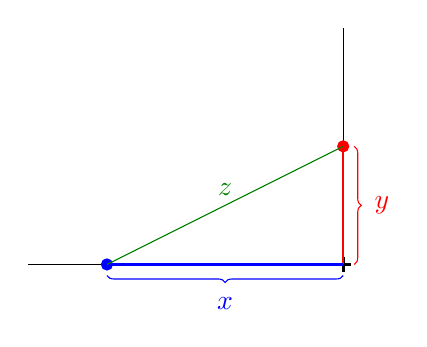
\begin{tikzpicture}[x=0.05cm, y=0.05cm]
            \draw (0, 60) -- (0, 0) -- (-80, 0);
            \draw[very thick] (2, 0) -- (-2, 0);
            \draw[very thick] (0, 2) -- (0, -2);
            \draw[red, fill=red] (0, 30) circle(2pt);
            \draw[blue, fill=blue] (-60, 0) circle(2pt);
            \draw[red, thick] (0, 0) -- (0, 30);
            \draw[blue, thick] (0, 0) -- (-60, 0);
            \draw[red, decorate, decoration={brace, mirror}, xshift=4pt] (0,
            0) -- node[midway, xshift=1em]{$y$} (0, 30);  
            \draw[blue, decorate, decoration={brace}, yshift=-4pt]
            (0, 0) -- node[midway, yshift=-1em]{$x$} (-60, 0);
            \draw[green!50!black] (0, 30) -- node[above]{$z$} (-60, 0);
          \end{tikzpicture}
        \end{center}
      }

      \ideas{Now, we try to relate variables.  In this case, since the
        rates we know about are $\frac{d\bm{x}}{dt}$ and
        $\frac{d\bm{y}}{dt}$, and the rate we want to know is
        $\frac{d\bm{z}}{dt}$, we try to relate $x$, $y$, and $z$.}

      We see a right triangle in our picture, so we can use the
      Pythagorean theorem to relate the lengths of its sides:

      \highlight{\textbf{Equation relating our variables:} $x^2 + y^2 =
        z^2$}

      \ideas{Once we have our relating equation, we differentiate it.
        Since we are looking for $\frac{dz}{d\bm{t}}$, we should
        differentiate it with respect to $t$.}

      Now, we differentiate the relating equation with respect to $t$,
      using implicit differentiation:
      \begin{align}
        \frac{d}{dt} (x^2 + y^2) &= \frac{d}{dt} (z^2) \nonumber \\
        2x \frac{dx}{dt} + 2y \frac{dy}{dt} &= 2z
        \frac{dz}{dt}
      \end{align}

      \ideas{Since we care about what happens at a specific moment, we can
        plug in our ``snapshot'' information.}

      At the moment we are interested in, $x = 80$, $y = 60$,
      $\dfrac{dx}{dt} = -30$, $\dfrac{dy}{dt} = -20$, and $z = 100$ by the
      Pythagorean Theorem.  Plugging this all in to the previous equation
      gives
      \[ 2 (80)(-30) + 2 (60)(-20) = 2 (100) \frac{dz}{dt},\] so
      $\dfrac{dz}{dt} = -36$.  In words, the distance between the cars is
      \begin{center}
        \fbox{decreasing at an instantaneous rate of 36 ft/s}.
      \end{center}
    \end{solution}

\item 
    \note{This will be quite challenging for students.  The first issue is
      that they see the formula $V = \frac{1}{3} \pi r^2 h$, want to plug
      in $r = 6$ and $h = 10$, and are then stuck.  They need to realize
      that there's something in the problem that's changing, and it's not
      the height of the cone!

      Students can also get tied up in knots about the fact that $V$
      depends on both $r$ and $h$.  Encourage them to keep the goal and
      known information in mind: they want to know
      $\frac{d\bm{h}}{dt}$ and they know $\frac{d\bm{V}}{dt}$,
      so it will be easier if they relate just $h$ and $V$ before
      differentiating.

      Matt note - I would at least set this problem up before class ends as their is a problem on the PSET very similar to it.
    }

    \begin{problem}[\vfill]
      An oil tank in the shape of an inverted cone has height 10 m and
      radius 6 m. When the oil is 5 m deep, the tank is leaking oil from
      the tip at a rate of 2 m$^3$ per day. How quickly is the height of
      the oil in the tank decreasing at this moment?

      \textit{Note:} The volume of a cone of radius $r$ and height $h$ is
      $\frac{1}{3} \pi r^2 h$.
    \end{problem}

    \begin{solution}
      \ideas{As usual, let's start by drawing two pictures, a generic
        picture that applies at any time, and a ``snapshot'' showing the
        situation at the time we care about.  We'll also label some
        variables in the generic picture (the things labeled in red are
        changing).}  

      \begin{center}
        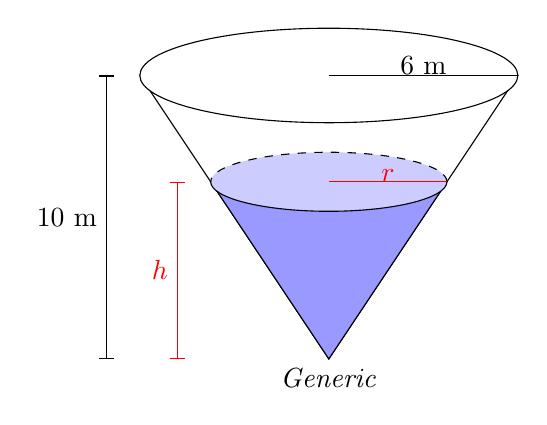
\begin{tikzpicture}[x=0.3cm, y=0.3cm]
          \def\R{8}
          \def\H{12}
          \def\r{5}
          \def\h{60/8}
          \def\aspect{4}
          \draw [fill=white] (-\R,\H) -- (\R,\H) -- (0,0) -- cycle;
          \draw [fill=white] (0, \H) circle [x radius=\R, y
          radius={\R/\aspect}];
          \draw [fill=blue!40!white,opacity=1] (-\r, \h) -- (\r, \h) --
          (0,0) -- cycle; 
          \draw [fill=blue!20!white,opacity=1, draw opacity=0] (0, \h) ellipse
          [x radius=\r, 
          y radius={\r/\aspect}];
          \draw (-\r, \h) arc [x radius=\r, y radius={\r/\aspect}, start
          angle=180, end angle=360];      
          \draw[dashed] (\r, \h) arc [x radius=\r, y radius={\r/\aspect},
          start angle=0, end angle=180];
          \draw (0, \H) -- node[above, inner sep=0.1pt]{6 m} (\R, \H);
          \draw[|-|, xshift=-12pt] (-\R, 0) -- node[left]{10 m} (-\R,
          \H);
          \draw[red] (0, \h) -- node[above, inner sep=0]{$r$} (\r, \h);
          \draw[red, |-|, xshift=-12pt] (-\r, 0) -- node[left]{$h$} (-\r,
          \h);
          \draw (0, 0) node[below, font=\normalsize]{\emph{Generic}};
        \end{tikzpicture} \hspace{0.5in}
        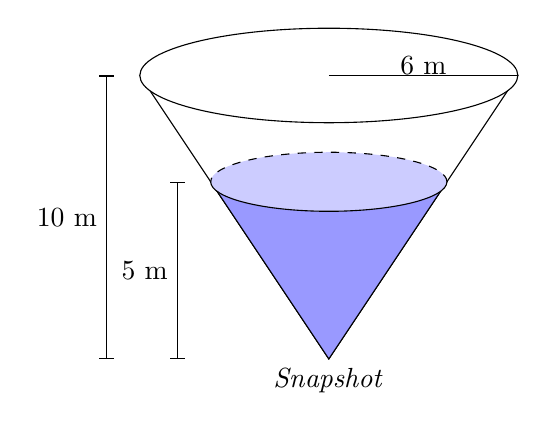
\begin{tikzpicture}[x=0.3cm, y=0.3cm]
          \def\R{8}
          \def\H{12}
          \def\r{5}
          \def\h{60/8}
          \def\aspect{4}
          \draw [fill=white] (-\R,\H) -- (\R,\H) -- (0,0) -- cycle;
          \draw [fill=white] (0, \H) circle [x radius=\R, y
          radius={\R/\aspect}];
          \draw [fill=blue!40!white,opacity=1] (-\r, \h) -- (\r, \h) --
          (0,0) -- cycle; 
          \draw [fill=blue!20!white,opacity=1, draw opacity=0] (0, \h) ellipse
          [x radius=\r, 
          y radius={\r/\aspect}];
          \draw (-\r, \h) arc [x radius=\r, y radius={\r/\aspect}, start
          angle=180, end angle=360];      
          \draw[dashed] (\r, \h) arc [x radius=\r, y radius={\r/\aspect},
          start angle=0, end angle=180];
          \draw (0, \H) -- node[above, inner sep=0.1pt]{6 m} (\R, \H);
          \draw[|-|, xshift=-12pt] (-\R, 0) -- node[left]{10 m} (-\R,
          \H);
          \draw[|-|, xshift=-12pt] (-\r, 0) -- node[left]{5 m} (-\r,
          \h);
          \draw (0, 0) node[below, font=\normalsize]{\emph{Snapshot}};
        \end{tikzpicture} 
      \end{center}
      Note that the radius and height of the tank are constant, but the
      radius and height of the oil change as oil leaks out, so we assign
      variables to those. 

      \ideas{Next, we figure out what we know and what we want to know.}

      \highlight{ \textbf{What we know:} If we let $V$ represent the
        volume of oil (in cubic m) at time $t$ (where $t$ is measured in
        days), then $\frac{dV}{dt} = -2$.  (This rate is negative because
        the volume is decreasing.)

        \textbf{What we want to know:} $\frac{dh}{dt}$ 
      }

      \ideas{Now, we try to relate variables.  In this case, since the rate
        we know is $\frac{d\bm{V}}{dt}$ and the rate we want to know is
        $\frac{d\bm{h}}{dt}$, we try to relate $V$ to $h$. }

      First, the volume $V$ of oil is the volume of a cone with radius $r$
      and height $h$, so $V = \frac{1}{3} \pi r^2 h$.  We'd like to get $V$
      in terms of just $h$, so we need to express $r$ in terms of $h$.
      Here, the key is similar triangles:
      \begin{center}
        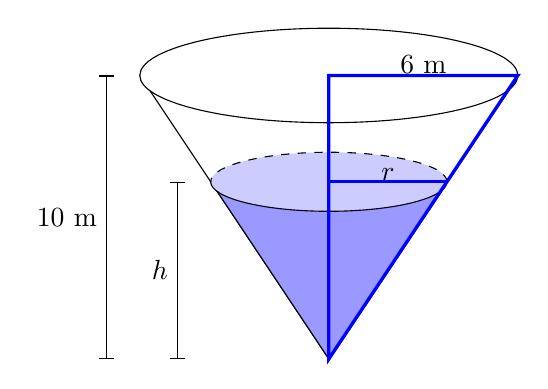
\begin{tikzpicture}[x=0.3cm, y=0.3cm]
          \def\R{8}
          \def\H{12}
          \def\r{5}
          \def\h{60/8}
          \def\aspect{4}
          \draw [fill=white] (-\R,\H) -- (\R,\H) -- (0,0) -- cycle;
          \draw [fill=white] (0, \H) circle [x radius=\R, y
          radius={\R/\aspect}];
          \draw [fill=blue!40!white,opacity=1] (-\r, \h) -- (\r, \h) --
          (0,0) -- cycle; 
          \draw [fill=blue!20!white,opacity=1, draw opacity=0] (0, \h) ellipse
          [x radius=\r, 
          y radius={\r/\aspect}];
          \draw (-\r, \h) arc [x radius=\r, y radius={\r/\aspect}, start
          angle=180, end angle=360];      
          \draw[dashed] (\r, \h) arc [x radius=\r, y radius={\r/\aspect},
          start angle=0, end angle=180];
          \draw[blue, very thick] (0, 0) -- (0, \H) --
          node[above, inner sep=0.1pt, black]{6 m}
          (\R, \H) -- cycle;      
          \draw[blue, very thick] (0, \h) -- node[above, inner sep=0,
          black]{$r$} (\r, \h); 
          \draw[|-|, xshift=-12pt] (-\R, 0) -- node[left]{10 m} (-\R,
          \H);
          \draw[|-|, xshift=-12pt] (-\r, 0) -- node[left]{$h$} (-\r,
          \h);
        \end{tikzpicture}
      \end{center}    
      From the similar triangles shown in blue, we get $\displaystyle
      \frac{6}{10} = \frac{r}{h}$, so $r = \dfrac{3 h}{5}$.  Plugging this
      into our equation for $V$, we get

      \highlight{\textbf{Equation relating our variables:} $\displaystyle V
        = \frac{1}{3} \pi \left( \frac{3h}{5} \right)^2 h = \frac{3
          \pi}{25} h^3$} 

      \ideas{Once we have our relating equation, we differentiate it.  Since
        we are looking for $\frac{dh}{d\bm{t}}$, we should differentiate
        with respect to $t$.}
      \begin{align}
        \frac{d}{dt} (V) &= \frac{d}{dt} \left( \frac{3 \pi}{25} h^3
        \right) \nonumber \\
        \frac{dV}{dt} &= \frac{9 \pi}{25} h^2 \frac{dh}{dt} \nonumber \\
        \intertext{At the moment we're interested in, $\frac{dV}{dt} = -2$
          and $h = 5$:}
        -2 &= \frac{9 \pi}{25} (25)
        \frac{dh}{dt}
 \nonumber 
      \end{align}
      So, $\displaystyle \frac{dh}{dt} = - \frac{2}{9 \pi}$.  So, at the
      time we're interested in, the height of oil is
      \begin{center}
        \fbox{decreasing at $\frac{2}{9 \pi}$ m/day}
      \end{center}
    \end{solution}

\item 
  \begin{problem}[\vfill]
    At noon, you are dashing through Harvard Yard to get to class and
    notice a friend 100 feet west of you, also running to class. If you
    are running south at a constant rate of 450 ft/min (approximately 5
    mph) and your friend is running north at a constant rate of 350 ft/min
    (approximately 4 mph), how fast is the distance between you and your
    friend changing at 12:02 pm?
  \end{problem}

  \begin{solution}
    \ideas{As usual, let's start by drawing two pictures, a generic
      picture that applies at any time, and a ``snapshot'' showing the
      situation at the time we care about.  We'll also label some
      variables in the generic picture.} 

    Between noon and 12:02, you run (450 ft/min)(2 min) = 900 ft, and your
    friend runs (350 ft/min)(2 min) = 700 ft. 
    \begin{center}
      \begin{tabular}{ccc}
        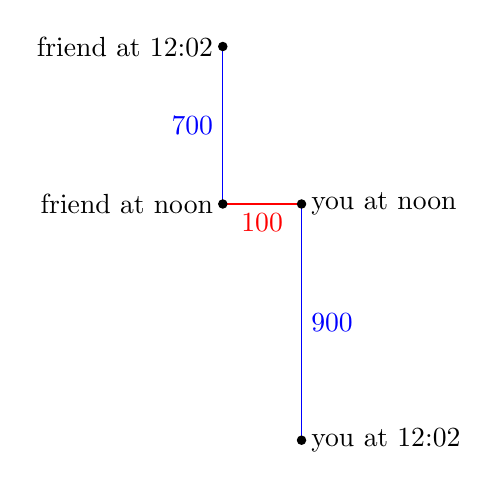
\begin{tikzpicture}
          \coordinate (FN) at (0, 0);
          \coordinate (YN) at (1, 0);
          \coordinate (Y) at (1, -3);
          \coordinate (F) at (0, 2);
          \draw[red] (FN) -- node[below]{100} (YN);
          \draw[blue] (YN) -- node[right]{900} (Y);
          \draw[blue] (FN) -- node[left] {700} (F);
          \filldraw (YN) circle(1.5pt) node[right]{you at noon};
          \filldraw (FN) circle(1.5pt) node[left] {friend at noon};
          \filldraw (F) circle(1.5pt) node[left] {friend at 12:02};
          \filldraw (Y) circle(1.5pt) node[right] {you at 12:02};
        \end{tikzpicture} & &
        \begin{tikzpicture}
          \coordinate (FN) at (0, 0);
          \coordinate (YN) at (1, 0);
          \coordinate (Y) at (1, -3);
          \coordinate (F) at (0, 2);
          \draw[green!80!black] (Y) -- node[right]{$z$} (F);
          \draw[blue] (F) -- (F |- Y);
          \draw[red] (F |- Y) -- node[below]{100} (Y);
          \filldraw (YN) circle(1.5pt) node[right]{you at noon};
          \filldraw (FN) circle(1.5pt) node[left] {friend at noon};
          \filldraw (F) circle(1.5pt) node[left] {friend at 12:02};
          \filldraw (Y) circle(1.5pt) node[right] {you at 12:02};
          \draw[blue, |-|] ($(F) + (3.5, 0)$) -- node[right]{$y$} ($(F |-
          Y) + (3.5, 0)$); 
        \end{tikzpicture} \\
        \textit{Snapshot (12:02)} & \hspace{0.25in} & \textit{Generic}  \\
      \end{tabular}
    \end{center}
    In the generic picture, we've let $z$ be the distance (in feet)
    between you and your friend and $y$ be the ``vertical'' (north-south)
    distance (in feet) between you and your friend.

    \ideas{Next, we figure out what we know and what we want to know.}

    \highlight{
      \textbf{What we know:} $\frac{dy}{dt} = 450 + 350 = 800$ ft/min

      \textbf{What we want to know:} $\frac{dz}{dt}$
    }

    \ideas{Now, we try to relate variables.  In this case, since the rates
      we know is $\frac{d\bm{y}}{dt}$ and the rate we want to know is
      $\frac{d\bm{z}}{dt}$, we try to relate $y$ and $z$.}
    Using our generic picture, we see that we can relate our variables
    using the Pythagorean Theorem:

    \highlight{\textbf{Equation relating our variables:} $y^2 + 100^2 =
      z^2$}  

    \ideas{Once we have our relating equation, we differentiate it.  Since
      we are looking for $\frac{dz}{d\bm{t}}$, we should differentiate
      with respect to $t$.}
    \begin{align*}
      \frac{d}{dt} \left( y^2 + 100^2 \right) &= \frac{d}{dt} \left( z^2
      \right) \\
      2y \frac{dy}{dt} &= 2z \frac{dz}{dt} \\
      \intertext{We can simplify this a bit by dividing through by 2:} % 
      y \frac{dy}{dt} &= z \frac{dz}{dt} \\
      \intertext{Now, we plug in the snapshot information and rate we
        know.  To get $z$ at the snapshot moment, we can use the
        Pythagorean Theorem (or the relation $y^2 + 100^2 = z^2$ that we
        got from using the Pythagorean Theorem earlier):} % 
      1600 (800) &= \sqrt{1600^2 + 100^2} \frac{dz}{dt} 
    \end{align*}
    So, $\displaystyle \frac{dz}{dt} = \frac{12800}{\sqrt{257}}$; that is,
    the distance between you and your friend is \fbox{increasing at
      $\dfrac{12800}{\sqrt{257}}$ ft/min} at 12:02.
  \end{solution}

\end{enumerate}

\end{document}